\chapter{CTMQC applied to the Tully Models}
\label{chap:tully_models}

The Tully models, first proposed by John Tully in 1990 \cite{tully_molecular_1990}, are a collection of model systems. They were designed to be simple enough to obtain accurate quantum results to benchmark new nonadiabatic molecular dynamics (NAMD) methods against. Originally there were 3, 1 dimensional, 1 atom models. However, both in Gossel, 18 \cite{gossel_coupled-trajectory_2018} and Agostini, 16 \cite{agostini_quantum-classical_2016} 1 new model was proposed (model 4) which is a logical extension of model 3. It is with these toy models that I will test my implementation of CTMQC and make comparisons to results in the literature.
\\\\
In each of the Tully models the (diabatic) Hamiltonian is defined by the nuclear positions and is a 2$\times$2 matrix that takes the form:
\[\hat{H} = \frac{\ \hat{P} \ ^2}{2M} + \left(
\begin{array}{cc}
  H_{11}(\mathbf{R}) & H_{12}(\mathbf{R}) \\
  H_{21}(\mathbf{R}) & H_{22}(\mathbf{R})
\end{array} \right)\]
The nuclear mass is set to 2000 AU, this was set to be very close to the proton's mass of 1836 AU so we can expect significant quantum effects that classical theory couldn't replicate. The values of the Hamiltonian elements are set to produce systems that resemble common features in a typical nonadiabatic simulation such as avoided crossings and regions of extended coupling. The exact parameters used can be found in the appendix \ref{app:tully_params}, though schematics of the 4 models can be found below in fig \ref{fig:tully_schematics}.

\begin{figure}[H]
  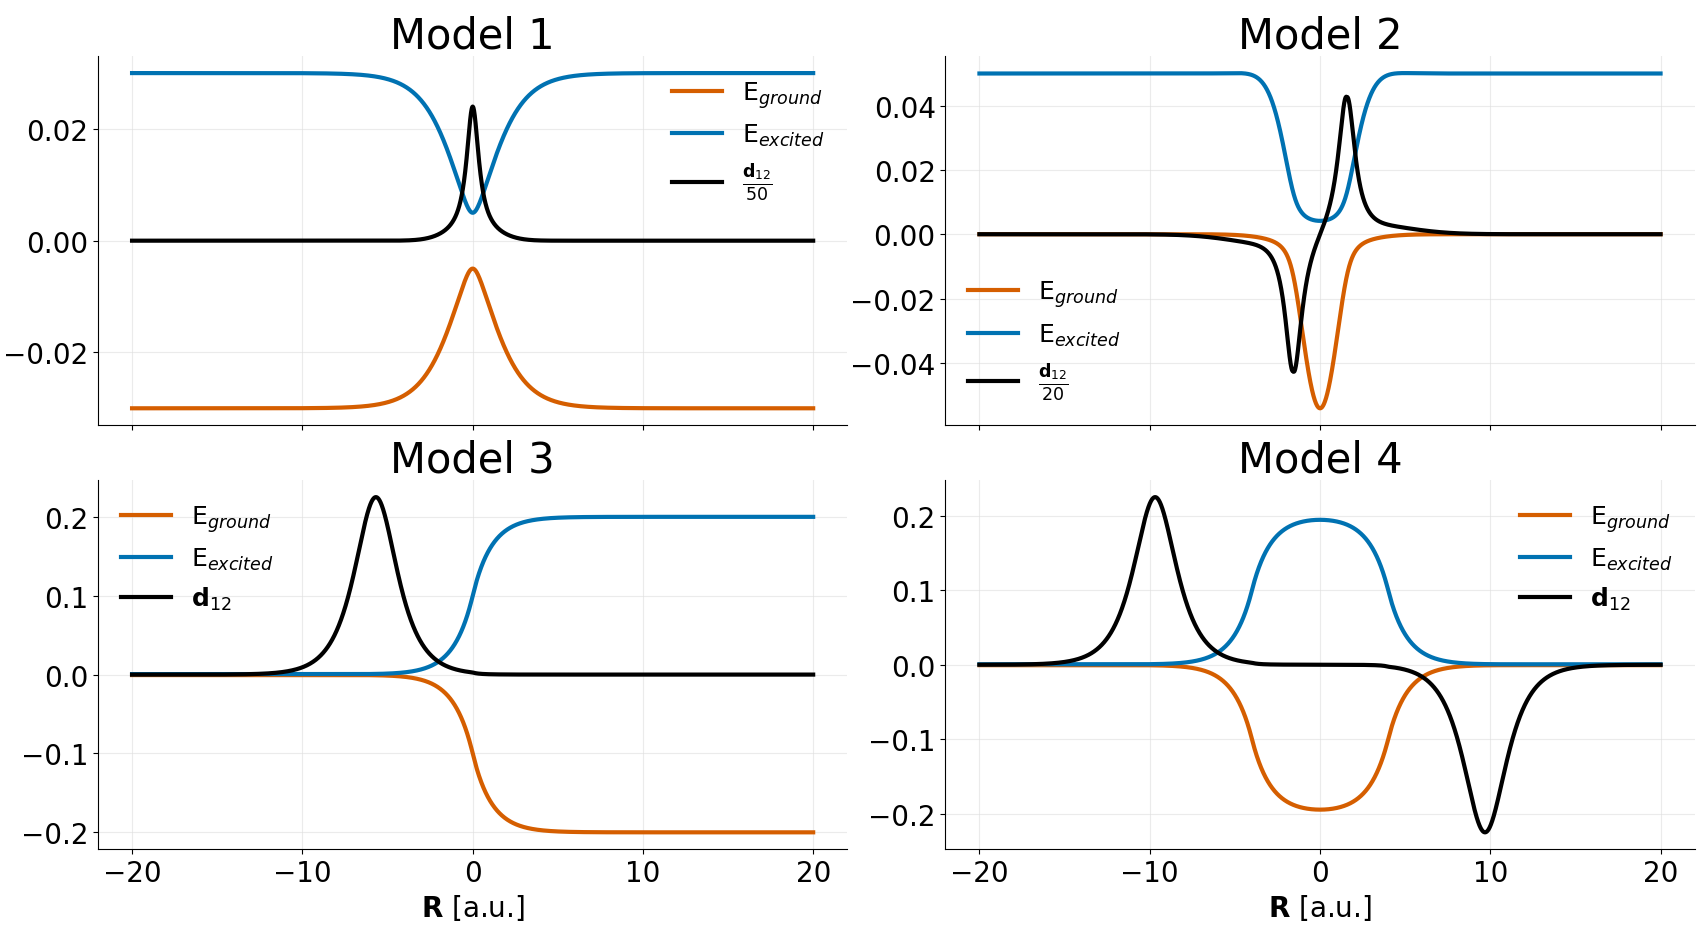
\includegraphics[width=\textwidth]{Chapter_tullyModels/model_schematics.png}
  \caption{\label{fig:tully_schematics}Adiabatic potential energy surfaces (orange and blue) and element 1, 2 of the nonadiabatic coupling vector for the 4 model systems. For parameters see appendix \ref{app:tully_params}.}
\end{figure}
